[8~r\textsuperscript{o}]
\pend
\count\Bfootins=1200
\count\Afootins=1200
%\newpage
\pstart
Si corpus aliquod grave descendens in aliud
\edtext{ipso gravius}{\lemma{ipso}\Bfootnote{\textit{(1)}\ celerius \textit{(2)}\ gravius \textit{L}}}
incidat, idque attollat,
(:~ponendo utrumque grave\protect\index{Sachverzeichnis}{grave} in punctum esse collectum
ne de mole ejus et inde orta retardatione\protect\index{Sachverzeichnis}{retardatio} sermo sit~:)
quaeritur quid 
\edtext{futurum sit. Ante omnia perinde erit, ac si differentia horum ponderum}{\lemma{futurum sit}\Bfootnote{\textit{(1)}\ ; an scilicet perinde sit ac si differentia horum duorum corporum \textit{(2)}\ . Ante [...] ponderum \textit{L}}}
sursum tendat: porro quaeritur qua celeritate\protect\index{Sachverzeichnis}{celeritas} horum ponderum differentia tendet sursum
\edtext{statim ab initio ictus\protect\index{Sachverzeichnis}{ictus}}{\lemma{}\Bfootnote{statim [...] ictus \textit{erg. L}}}.
An ea ipsa quae fuit impingentis in illo momento. An vero ea quae
\edtext{est in reciproca ratione differentiae}{\lemma{est}\Bfootnote{\textit{(1)}\ differentiae \textit{(2)}\ in [...] differentiae \textit{L}}}
ad impingens? De ipsis quoque continuis incrementis quaestio est
\edtext{rursus.\\\hspace*{7,5mm}Grave quod motu acceleratione quaesito movetur, habet vim suam compositam ex aggregato repetitionum, ac proinde est ad vim primam, ut linea est ad aliquod punctum seu lineam infinite parvam. Prout grave illud punctum}{\lemma{rursus.}\Bfootnote{\textit{(1)}\ Nempe si grave aliquod in punctum collectum \textit{(2)}\ Grave [...] habet  \textit{(a)}\ momentum suum factum ex vi ipsa qua impelli  \textit{(b)}\ vim [...] parvam.  \textit{(aa)}\ Esto  \textit{(bb)}\ Prout [...] punctum \textit{L}}}
ab initio valde vel parum grave
\edtext{est, gravitationem ejus appellemus $\displaystyle g.$}{\lemma{est,}\Bfootnote{\textit{(1)}\ vim primam appellemus $\displaystyle b$ vel tempus \textit{(2)}\ numerum instantium temporis seu repetitionum \textit{(3)}\ gravitatem \textit{(4)}\ gravitationem ejus appellemus\ \textit{(a)}\ $\displaystyle p.$\  \textit{(b)}\ $\displaystyle g.$ \textit{L}}}
celeritatem qua initio tendit,
\edtext{vocabimus $\displaystyle c.$}{\lemma{vocabimus}\Bfootnote{\textit{(1)}\ $\displaystyle t.$ \textit{(2)}\ $\displaystyle c.$ \textit{L}}}
erit vis ejus prima
\edtext{$\displaystyle gc$. Nam}{\lemma{$\displaystyle gc$.}\Bfootnote{\textit{(1)}\ et vis e \textit{(2)}\  et  \textit{(a)}\ si \textit{(b)}\ tempus  \textit{(aa)}\ percurs \textit{(bb)}\ quo descendit a \textit{(3)}\ Nam \textit{L}}}
exempli causa si grave conetur oblique ut in plano inclinato\protect\index{Sachverzeichnis}{planum inclinatum},
eadem erit celeritas ab initio,
\edtext{at gravitatio}{\lemma{at}\Bfootnote{\textit{(1)}\ gravitas \textit{(2)}\ gravitatio \textit{L}}} diversa
\edtext{ita si plumbea sit vel lignea}{\lemma{}\Bfootnote{ita si  \textit{(1)}\ numerus \textit{(2)}\ plumbea sit vel lignea \textit{erg.} \textit{L}}}.
Jam durante motu celeritates repetuntur sive ictus, unde cum
\edtext{sit primo momento $\displaystyle g, 1c$, secundo $\displaystyle g, 2c$, tertio}{\lemma{sit}\Bfootnote{%
\textit{(1)}\ ab ini %
\textit{(2)}\ primo momento %
\textit{(a)}\ $\displaystyle 1cg.$ secundo $\displaystyle 2c \smallfrown g$ tertio %
\textit{(b)}\ $\displaystyle g, 1c$, [...] tertio \textit{L}}}
$\displaystyle g, 3c$ etc. \rule[-4mm]{0mm}{10mm}
\edtext{erit generaliter}{\lemma{erit}\Bfootnote{\textit{(1)}\ denique post m \textit{(2)}\ generaliter \textit{L}}}
\edtext{$\displaystyle g,\frac{t}{a}c$, numerum}{\lemma{$\displaystyle g,\frac{t}{a}c$,}\Bfootnote{\textit{(1)}\ magnitudinem \textit{(2)}\ numerum \textit{L}}}
momentorum seu temporis tractum vocando %\rule[-4mm]{0mm}{10mm}
$\displaystyle \frac{t}{a}$.
Jam in itinere aliud occurrat gravitans, cujus gravitatio ad gravitationem primi rationem habeat datam, sit ergo \rule[-4mm]{0mm}{10mm}
\edtext{$\displaystyle \frac{d}{a}g$. Resistentia ejus est composita ex gravitate, et celeritate qua levari debet. Experientia enim constat gravia levanda resistere in ratione celeritatum quibus levari debent. Ergo resistentia ejus erit $\displaystyle \frac{d}{a}gtc$.}{\lemma{$\displaystyle \frac{d}{a}g$}\Bfootnote{\textit{(1)}\ , erit ejus resistentia prima $\displaystyle \frac{d}{a}g1c$ \textit{(2)}\ . Resistentia [...]  gravia  \textit{(a)}\ celerius leve  \textit{(b)}\ levanda [...] $\displaystyle \frac{d}{a}gtc$. \textit{L}}}
\rule[-4mm]{0mm}{10mm} Ergo vis residua, subtracta resistentia erit  $\displaystyle g,\frac{t}{a}c, \smallfrown \frac{a-d}{a}$.
Quod si \edtext{celeritas}{\lemma{si}\Bfootnote{\textit{(1)}\ tempus \textit{(2)}\  celeritas \textit{L}}}
non fuisset ut $\displaystyle \frac{t}{a}c$,
sed alia, v.g. $\displaystyle \frac{\theta}{a}c$,
foret vis residua \rule[-4mm]{0mm}{10mm} $\displaystyle g,\frac{\theta}{a}c,\smallfrown\frac{a-d}{a}$.
quae est ad priorem ut $\displaystyle \frac{t}{a}c$, ad $\displaystyle \frac{\theta}{a}c$.
seu in ratione \edtext{celeritatum. Virium quoque diminutiones}{\lemma{celeritatum.}\Bfootnote{\textit{(1)}\ Jam \textit{(2)}\ Ergo et \textit{(3)}\ Virium quoque diminutiones \textit{L}}}
\rule[-4mm]{0mm}{10mm} $\displaystyle \frac{d}{a}g,\frac{t}{a}c$,
item \rule[-4mm]{0mm}{10mm} $\displaystyle \frac{d}{a}g,\frac{\theta}{a}c$
erunt ut eaedem celeritates seu ut $\displaystyle t$ ad $\displaystyle \theta$.
Ergo et virium diminutiones erunt ut celeritates;
ergo cum \edtext{non gravitatio}{\lemma{}\Bfootnote{non  \textbar\ nisi \textit{gestr.}\ \textbar\ gravitatio \textit{L}}}
sed celeritas minuatur erunt et celeritatum diminutiones, ut celeritates.
Sed ex hoc calculo videtur sequi falsum.
Nam si $\displaystyle d$ ponatur $\displaystyle \sqcap \, a$ fiet celeritas nulla, quod tamen falsum est.
Nam etiam majus corpus a minore in ipsum cadente elevatur.
Non ergo resistit grave ea celeritate qua elevandum est;
alioquin majus a minore non elevaretur, nec pendulum elevaret seipsum celeritate
\edtext{quaesita. Resistentia ergo}{\lemma{quaesita.}\Bfootnote{\textit{(1)}\ Non ergo \textit{(2)}\ Resistentia ergo \textit{L}}}
ponderis \rule[-4mm]{0mm}{10mm} $\displaystyle \frac{d}{a}g$ erit $\displaystyle \frac{d}{a}g,1c$.
et cum \edtext{ad aliquod tempus}{\lemma{ad}\Bfootnote{\textit{(1)}\ aliquam altitudinem \textit{(2)}\ aliquod tempus \textit{L}}}
elevatum erit, $\displaystyle \text{\hebr{t}}$,
quaesita intelligetur resistentia (id est detractum erit priori) illius \rule[-4mm]{0mm}{10mm}
$\displaystyle \frac{d}{a}g,\frac{\text{\hebr{t}}}{a}c$.
Id autem quod descendit, interea et ipsum acceleratum est, et erit
\pend
\pstart
\centering

 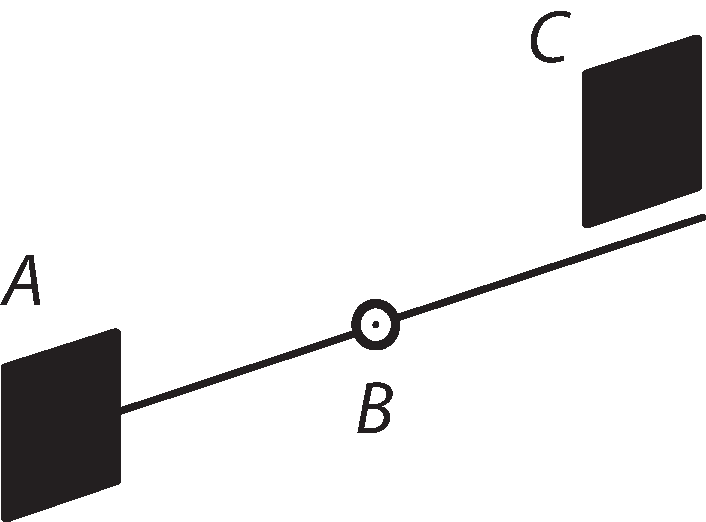
\includegraphics[trim = 0mm -3mm 0mm 0mm, clip, width=0.26\textwidth]{images/lh0350911_008r-d1.pdf}\\
\centering [\textit{Fig. 6}] % \caption{Bildbeschreibung}
\pend
\vspace{1em}
\pstart
\noindent ejus \setline{1}vis quaesita:\rule[-4mm]{0mm}{10mm} $\displaystyle g,\frac{t+\text{\hebr{t}}}{a}c$.
Tum ergo \edtext{quiescet compositum}{\lemma{quiescet}\Bfootnote{\textit{(1)}\ corpus, cum p \textit{(2)}\ compositum \textit{L}}}
ex utroque cum fiet:
$\displaystyle \ovalbox{$g,\!$}\, \frac{t+\text{\hebr{t}}}{a} \, \underset{\scriptscriptstyle{I\!\!I}}{\smash[b]{\ovalbox{$c$}}} \, ,\!, - \, \frac{d}{a} \,\ovalbox{$g$} \, , \frac{\text{\hebr{t}}}{a} \,\underset{\scriptscriptstyle{I\!\!I}}{\smash[b]{\ovalbox{$c$}}} \ \sqcap \ 0$.
seu $\displaystyle t + \text{\hebr{t}} - \frac{d \, \text{\hebr{t}}}{a} \ \sqcap \ 0$.
sive $\displaystyle at + a \text{\hebr{t}} - d \text{\hebr{t}}$
\edtext{[$\displaystyle \sqcap \ 0$]}{\lemma{}\Bfootnote{$\displaystyle \ \sqcap \ 0$ \textit{erg. Hrsg.}}}. seu ponendo $\displaystyle d \, \sqcap \, e + a$,
fiet: $\displaystyle at + \ovalbox{$a \text{\hebr{t}}$}\, - e \text{\hebr{t}} \ \ovalbox{$-a \text{\hebr{t}}$} \ \sqcap \, 0$. adeoque $\displaystyle \frac{a}{e} \, \sqcap \, \frac{\text{\hebr{t}}}{t}$.
% \begin{wrapfigure}[7]{l}{0.3\textwidth}
%\vspace*{-8mm}
%    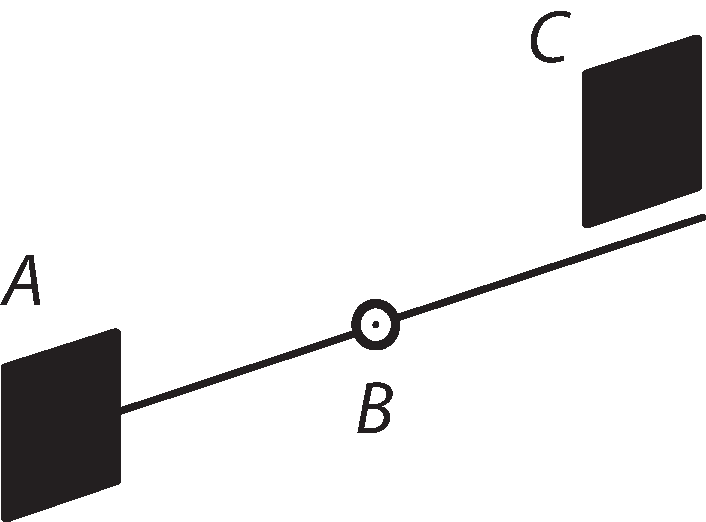
\includegraphics[trim = 0mm -3mm -5mm 0mm, clip, width=0.3\textwidth]{images/lh0350911_008r-d1.pdf}
%    \centering [\textit{Fig. 6}] % \caption{Bildbeschreibung}
%   \end{wrapfigure}
seu \rule[-4mm]{0mm}{10mm}\edtext{cum ponderum}{\lemma{cum}\Bfootnote{\textit{(1)} pondera \textit{(2)} ponderum \textit{L}}}
differentiae, \edtext{et tempora ante concursum, reciproce proportionalia}{\lemma{et}\Bfootnote{\textit{(1)} celeritates reciproce pro spa \textit{(2)} tempora  \textit{(a)} primum \textit{(b)} ante [...] proportionalia \textit{L}}}
\edtext{erunt. Nimirum}{\lemma{erunt.}\Bfootnote{%
\textit{(1)} Sed qui fit %
\textit{(2)} Quod %
\textit{(3)} Gravia resistere alias constat pro ratione celeritatis, qua levanda sunt. %
\textit{(4)} Nimirum \textit{L}}} idem contingit, ac si $\displaystyle A$ descendens circa centrum $\displaystyle B$ linea rigida $\displaystyle AB$ occurreret ipsi $\displaystyle C$ ponderi quiescenti elevando. Itaque hinc jam apparet resistentias non esse ut celeritates
\edtext{mutationum. Hic}{\lemma{mutationum.}\Bfootnote{\textit{(1)} Ratio \textit{(2)} Hic \textit{L}}}
$\displaystyle A$ et $\displaystyle C$ moventur aequivelociter.
Quare si solo unius gravitatis\protect\index{Sachverzeichnis}{gravitas} ictu moverentur esset quiescendum in casu aequalitatis.
Sed undulatio liquidi circumfusi, cui solus obstat motus gravitatis ipsius $\displaystyle C$ eo utique fortior est,
\edtext{quia undulatio illa est aggregatum gravitationum innumerabilium}{\lemma{quia}\Bfootnote{\textit{(1)} ipsemet est plurium undulationum \textit{(2)} undulatio [...] innumerabilium. \textit{L}}}.
Hinc jam porro sequitur si pondus $\displaystyle C$
seu \rule[-4mm]{0mm}{10mm} $\displaystyle \frac{d}{a} g$ sit minus quam pondus $\displaystyle g$
seu si $\displaystyle d \; \kleiner \, a$.  
nunquam inde sequetur quies,
\edlabel{035,09,11_008r_zz-1}%
\edtext{}{\xxref{035,09,11_008r_zz-1}{035,09,11_008r_zz-2}{\lemma{sed}\Bfootnote{%
\textit{(1)} vis %
\textit{(2)} fiet %
\textit{(a)} $\displaystyle g, \frac{t}{a} c \, - \, \frac{d}{a} g, c$ %
\textit{(b)} $\displaystyle g,\!, \smallfrown$ [...] $\displaystyle - \frac{d}{a} g, 1c.$ \textit{L}}}}%
sed fiet $\displaystyle g,\!, \smallfrown {\atop \lefthalfcup} \frac{t}{a} + 1 \! {\atop \righthalfcup} \, c,\!,\!, - \frac{d}{a} g, 1c.$%
\edlabel{035,09,11_008r_zz-2} Cum ergo%\pend